\section{Functionality of extension}
\label{sec:features}
The HLASM Language Support extension parses and analyzes all parts of a HLASM program. It resolves all ordinary symbols, variable symbols and checks the validity of most instructions. The extension supports conditional and unconditional branching and can define global and local variable symbols. It can also expand macros and COPY instructions.

\subsection{Highlighting}
The HLASM Language Support extension highlights statements with different colors for labels, instructions, operands, remarks and variables. Statements containing instructions that can have operands are highlighted differently to statements that do not expect operands. Code that is skipped by branching AIF, AGO or conditional assembly is not colored.

\begin{figure}[h]
	\centering
	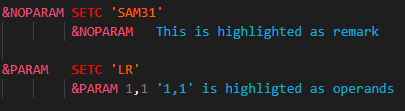
\includegraphics[width=10cm]{img/highligting}
	\caption{HLASM code with syntax highlighting.}
\end{figure}

\subsection{Autocomplete}
Autocomplete is enabled for the instruction field. While typing, a list of instructions starting with the typed characters displays. Selecting an instruction from the list completes it and inserts the default operands. Variables and sequence symbols are also filled with a value from their scope.

\begin{figure}[H]
	\centering
	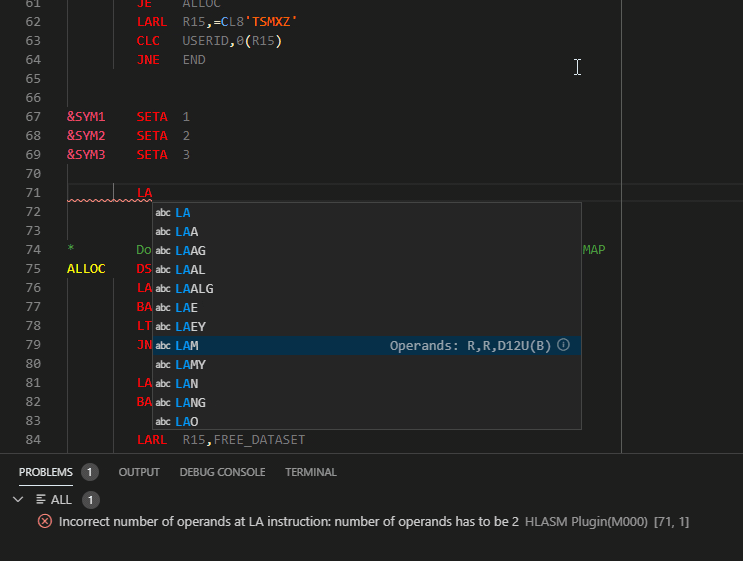
\includegraphics[width=\linewidth]{img/autocomplete/autocomplete-32}
	\caption{Autocomplete usage example.}
\end{figure}

\subsection{Go To Definition and Find All References}
The extension adds the functionality of \TT{go to definition} and \TT{find all references}. Use the \TT{go to definition} functionality to show definitions of variable symbols, ordinary symbols and macros, or open COPY files directly. Use the \TT{find all references} functionality to show all places where a symbol is used.

\begin{figure}[H]
	\centering
	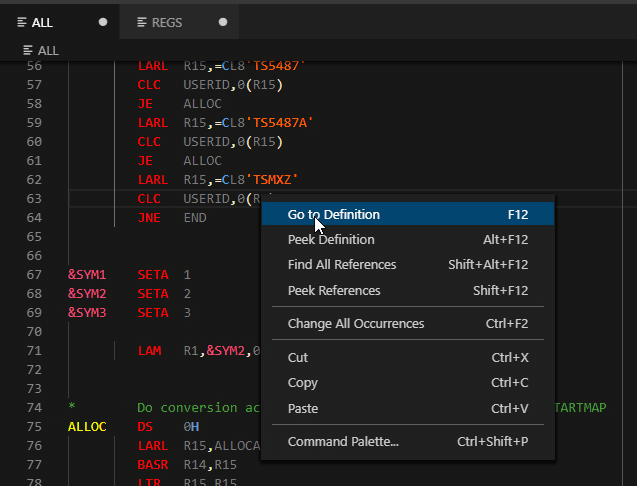
\includegraphics[width=.45\linewidth]{img/go_to_def/go_to_def-54}
	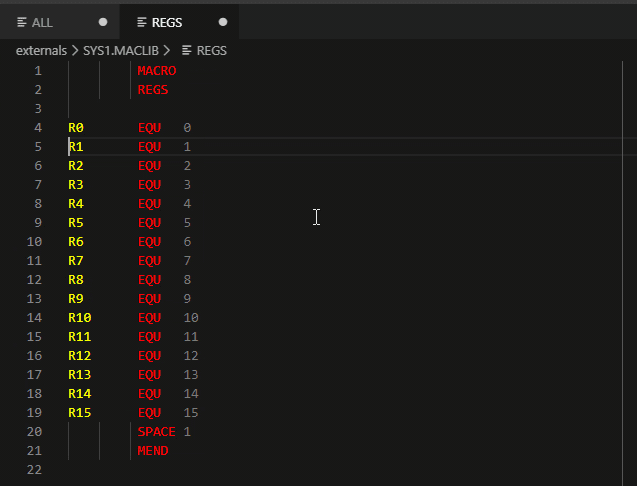
\includegraphics[width=.45\linewidth]{img/go_to_def/go_to_def-56}
	\caption{Go To Definition usage example; the editor opens the place of definition of the selected R1 symbol.}
\end{figure}

\subsection{Macro Tracer}
The macro tracer functionality allows you to track the process of assembling HLASM code. It lets you see step-by-step how macros are expanded and displays values of variable symbols at different points during the assembly process. You can also set breakpoints in problematic sections of your conditional assembly code. 

The macro tracer is not a debugger. It cannot debug running executables, only track the compilation process.

\subsubsection{Configuring the Macro Tracer}

\begin{enumerate}
	\item Open your workspace.
	\item In the left sidebar, click the bug icon to open the debugging panel (Ctrl + Shift + D).
	\item Click create a launch.json file. A \TT{select environment} prompt displays.
	\item Enter \textbf{HLASM Macro tracer}. Your workspace is now configured for macro tracing.
\end{enumerate}

\subsubsection{Using the Macro Tracer}

To run the macro tracer, open the file that you want to trace. Then press \textbf{F5} to open the debugging panel and start the debugging session.

When the tracer stops at a macro or COPY instruction, you can select \textbf{step into} to open the macro or COPY file, or \textbf{step over} to skip to the next line.

Breakpoints can be set before or during the debugging session.

\begin{figure}[H]
	\centering
	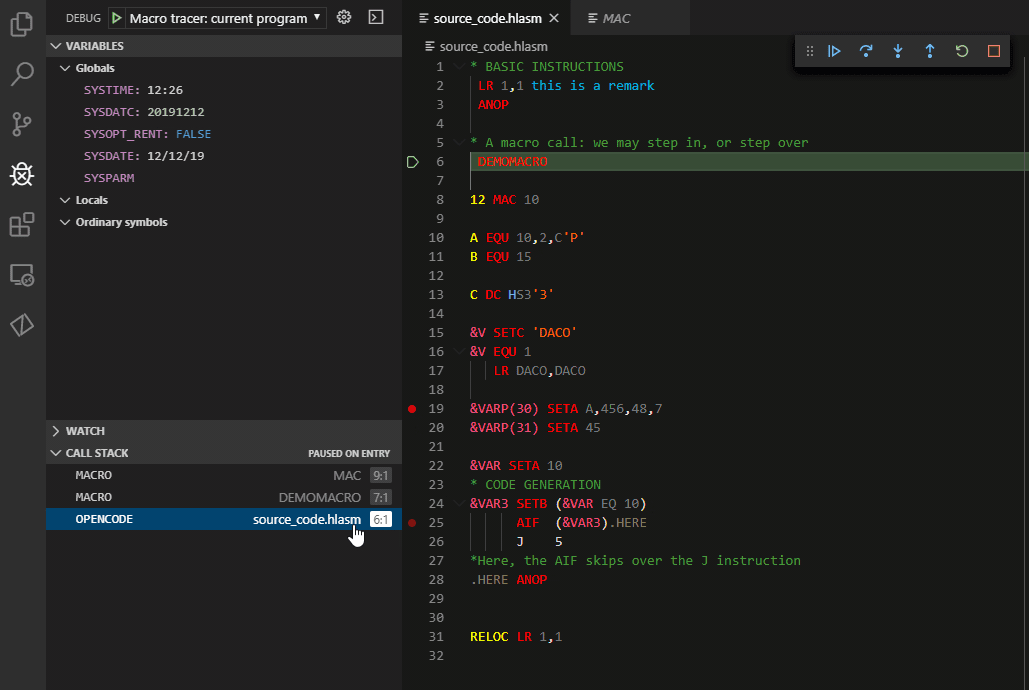
\includegraphics[width=\linewidth]{img/tracer/tracer-175}
	\caption{Macro tracer interface, showing HLASM source code with highlighted current instruction, call stack and variable listing.}
\end{figure}
